\documentclass{beamer}

\usepackage{amsmath}
\usepackage{graphicx}
\usepackage{tikz}
\usetikzlibrary{shapes.geometric, arrows}

\usetheme{Madrid}

\tikzstyle{startstop} = [rectangle, rounded corners, text centered, text width=2cm, draw=black, fill=red!30]
\tikzstyle{io} = [trapezium, trapezium left angle=70, trapezium right angle=110, text centered, draw=black, fill=blue!30]
\tikzstyle{process} = [rectangle, text centered, draw=black, fill=orange!30, text width=2cm]
\tikzstyle{decision} = [diamond, minimum width=3cm, minimum height=1cm, text centered,
draw=black, fill=green!30]
\tikzstyle{arrow} = [thick,->,>=stealth]
\tikzstyle{line} = [thick, -]

%\setlength{\parskip}{\baselineskip}

\AtBeginSection[]{
  \begin{frame}
  \vfill
  \centering
  \begin{beamercolorbox}[sep=8pt,center,shadow=true,rounded=true]{title}
    \usebeamerfont{title}\insertsectionhead\par%
  \end{beamercolorbox}
  \vfill
  \end{frame}
}

\title{
Quantum \textsc{Espresso}
}

\subtitle[]{
Guide to running simulations for DLS Spectroscopy
}

\author[J D Elliott]{
\footnotesize
Joshua D Elliott
}

\institute[DLS Ltd.]{
Diamond Light Source Ltd.
}

\date[V0.1 2022]{
\footnotesize
Updated: \today
}

%\begin{frame}
%\footnotesize
%\frametitle{}
%\framesubtitle{}
%\end{frame}

%%% OUTLINE %%%

% 1. Introduction to Quantum Espresso Code
%    - Concept
%    - Licence
%    - Help
%    - What Quantum Espresso is
% 2. Density Functional Theory
%    - QM with Density 
%    - KS Equation
%    - Self consistency cyle
%    - Self consistency in the output
%    - Representing quantities on a computer

\begin{document}

\frame{\titlepage}

\section{Introduction}

\subsection{What is Quantum \textsc{Espresso}}

\begin{frame}
\footnotesize
\frametitle{Quantum \textsc{Espresso}}
\framesubtitle{opEn Source Package for Research in Electronic Structure
Simulations and Optimization}

\begin{center}
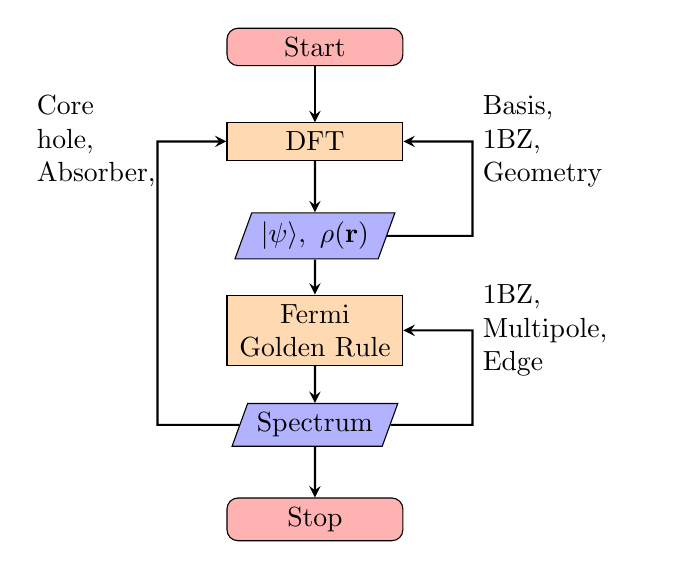
\begin{tikzpicture}[node distance=1.2cm]
\node (start) [startstop]
	{Start};
\node (dft) [process, below of=start]
	{DFT};
\node (wfn) [io, below of=dft]
	{$\vert \psi \rangle,\ \rho(\mathbf{r})$}; 
\node (fgr) [process, below of=wfn]
	{Fermi Golden Rule};
\node (spectrum) [io, below of=fgr]
	{Spectrum};
\node (stop) [startstop, below of=spectrum]
	{Stop} ;

\node (backwfn) [right of=wfn, xshift=1cm]{};
\node (backdft) [above of=backwfn]{};

\draw [arrow] (start) -- (dft);
\draw [arrow] (dft) -- (wfn);
\draw [arrow] (wfn) -- (fgr);
\draw [arrow] (fgr) -- (spectrum);
\draw [arrow] (spectrum) -- (stop);

\draw [arrow] (wfn) -- ++ (2cm,0)  |- node[text width=2cm, anchor=west]{Basis,\\ 1BZ,\\ Geometry} (dft);
\draw [arrow] (spectrum) -- ++(2cm,0) |- node[text width=2cm, anchor=west]{1BZ,\\ Multipole, \\ Edge}(fgr);
\draw [arrow] (spectrum) -- ++(-2cm,0) |- node[text width=1.4cm, anchor=east]{Core hole,\\ Absorber,}(dft);


\end{tikzpicture}
\end{center}

\end{frame}



\begin{frame}
\footnotesize
\frametitle{Open Source Software Package}



\end{frame}


\begin{frame}
\footnotesize
\frametitle{Where to get help?}

\alert{\textbf{At Diamond}}:\\
Email: joshua.elliott@diamond.ac.uk; Office: 1.12 Z02 (Ring); Ext:\\
Email: mihai.duta@diamond.ac.uk (installation/compilation problems)\\~\\

\textbf{Online}:\\
Web-site: www.quantum-espresso.org\\~\\

\textbf{Literature}:\\
Journal of Physics: Condensed Matter 2009, 21 (39), 395502.\\
Journal of Physics: Condensed Matter 2017, 29 (46), 465901.\\
Journal of Chemical Physics 2020, 152 (15), 154105.\\~\\

\textbf{Source Code}:\\
Doc folder under quantum espresso distribution\\~\\

\textbf{Mailing List}:\\
Email: users@lists.quantum-espresso.org\\
Archive of questions/issues dating back to 2011.\\
Web-site: https://www.mail-archive.com/users@lists.quantum-espresso.org/
\end{frame}

\begin{frame}
\footnotesize

\frametitle{A Software Suite}

Important: QE is not a single executable file, rather a collected distribution of several
executable programs.\\

\begin{center}
\begin{minipage}{0.85\textwidth}
\begin{tiny}
\begin{itemize}
   \item[\alert{PWscf}] Ground state electronic structure, structural optmiziation.
   \item[CP] Carr-Parrinello molecular dynamics.
   \item[PHonon] Linear-repsonse calculations.
   \item[\alert{PostProc}] Post processing, graphs and visualization.
   \item[PWneb] Nudged-Elastic Band driver from reaction paths.
   \item[atomic] Generation of pseudopotentials.
   \item[PWGui] Graphical User Interface for input.
   \item[PWcond] Ballistic conductance calculations.
   \item[\alert{XSpectra}] Core-level excitation spectra based on Fermi-Golden Rule.
   \item[GWL] Quasiparticle and Exciton energies based on GW/BSE approximation.
   \item[TD-DFPT] Time-dependent Density Functional Perturbation Theory.
   \item[EPW] Electron-phonon coupling.
   \item[HP] Automation of linear-response DFT+U parameters. 
\end{itemize}
\end{tiny}
\end{minipage}
\end{center}

All these packages and others share: (i) installation method, (ii) input file format,
(iii) pseudopotential file format, (iv) output format (v) source code.

\end{frame}

\section{Density Functional Theory - Theory}

\begin{frame}
\footnotesize
\frametitle{Quantum mechanics in terms of the electron density}

\onslide<1->{The total energy of the ground state of a system of electrons may be written as a
functional of the electron density.}

\begin{equation}
\onslide<1->{E^\mathrm{DFT}[n]; \hspace{2cm} 
\int n(\mathbf{r})\ \mathrm{d}\mathbf{r} = N; \hspace{2cm} 
n(\mathbf{r}) \ge 0}
\end{equation}

\onslide<2->{We can prove mathmatically that the functional exists, but the form is unknown. Within
Kohn-Sham formalism we write the functional:}

\onslide<2->{
\begin{equation}
E^\mathrm{DFT}[n] = T_s[\{\psi_i\}] + E_\mathrm{ext}[n] + E_\mathrm{Hartree}[n] +
E_{xc}[n] + E_\mathrm{ions}
\end{equation}
}

\onslide<3->{Within the functional we introduced the set of single particle orbitals $\{\psi_i\}$,
which are related to the density} 

\onslide<3->{
\begin{equation}
n(\mathbf{r}) = \sum_i^M \vert \psi_i(\mathbf{r}) \vert^2
\end{equation}
}

\onslide<4->{These are used to approximate the kinetic energy}
\onslide<4->{
\begin{equation}
T_s[\{\psi_i\}] = -\frac{1}{2} \sum_i^N \int \mathrm{d}\mathbf{r}\ \psi_i^*(\mathbf{r})
\nabla^2 \psi_i(\mathbf{r})
\end{equation}
}

\end{frame}

\begin{frame}
\footnotesize
\frametitle{Quantum mechanics in terms of the electron density}

\onslide<1->{The other terms are functionals of the density:

\begin{equation}
E_\mathrm{ext}[n] = \int \mathrm{d}\mathbf{r}\ n(\mathbf{r})V_\mathrm{ext}(\mathbf{r}),
\end{equation}

\begin{equation}
E_\mathrm{Hartree}[n] = \frac{1}{2} \int \mathrm{d}\mathbf{r} \mathrm{d}\mathbf{r}^\prime\
\frac{n(\mathbf{r})n(\mathbf{r}^\prime)}{\vert \mathbf{r} - \mathbf{r}^\prime \vert},
\end{equation}
}

\onslide<2->{The Ionic term is the pairwise interaction of the charged nuclei

\begin{equation}
E_\mathrm{ions} = \sum_{I,J\ne I} \frac{Z_I Z_J}{\vert \mathbf{R}_I - \mathbf{R}_J \vert}
\end{equation}

There difficulty with the approach lies in the exchange-correlation energy, whose form
remains unknown.
}

%\onslide<3->{
%Minimization of the functional derivitive of $E^\mathrm{DFT}$ with respect to the density
%$n$ gives

%\begin{equation}
%H^\mathrm{KS} \psi_i(\mathbf{r}) = 
%\left [ 
%-\frac{1}{2}\nabla^2 + V_\mathrm{ext}(\mathbf{r}) + V_\mathrm{Hartree}(\mathbf{r}) +
%V_{xc}(\mathbf{r}) 
%\right ] \psi_i(\mathbf{r}) = \varepsilon_i \psi_i(\mathbf{r})
%\end{equation}
%}
\end{frame}

\begin{frame}
\footnotesize
\frametitle{The Kohn-Sham Equations}

\onslide<1->{
Minimization of the functional derivitive of $E^\mathrm{DFT}$ with respect to the density
$n$ gives

\begin{equation}
H^\mathrm{KS} \psi_i(\mathbf{r}) = 
\left [ 
-\frac{1}{2}\nabla^2 + V_\mathrm{ext}(\mathbf{r}) + V_\mathrm{Hartree}(\mathbf{r}) +
V_{xc}(\mathbf{r}) 
\right ] \psi_i(\mathbf{r}) = \varepsilon_i \psi_i(\mathbf{r})
\end{equation}
}

\onslide<2->{
\begin{tiny}
\begin{equation}
V_\mathrm{Hartree} = 
\int \mathrm{d}\mathbf{r}^\prime\ 
\frac{n(\mathbf{r}^\prime)}{\vert \mathbf{r} - \mathbf{r}^\prime \vert } 
\end{equation}
\begin{equation}
V_{xc} = \frac{\delta E_{xc}}{\delta n}
\end{equation}
\end{tiny}
}

\onslide<3->{
The solutions of the Kohn-Sham equations are a set of states and energy levels spanning at
least the number of electrons in the system.\\~\\
}

\onslide<4->{
The issue with the formalism is that the Hamiltonian depends explicity on the orbitals and
density.
}

\end{frame}

\begin{frame}
\tiny
\frametitle{The self-consistency cycle}

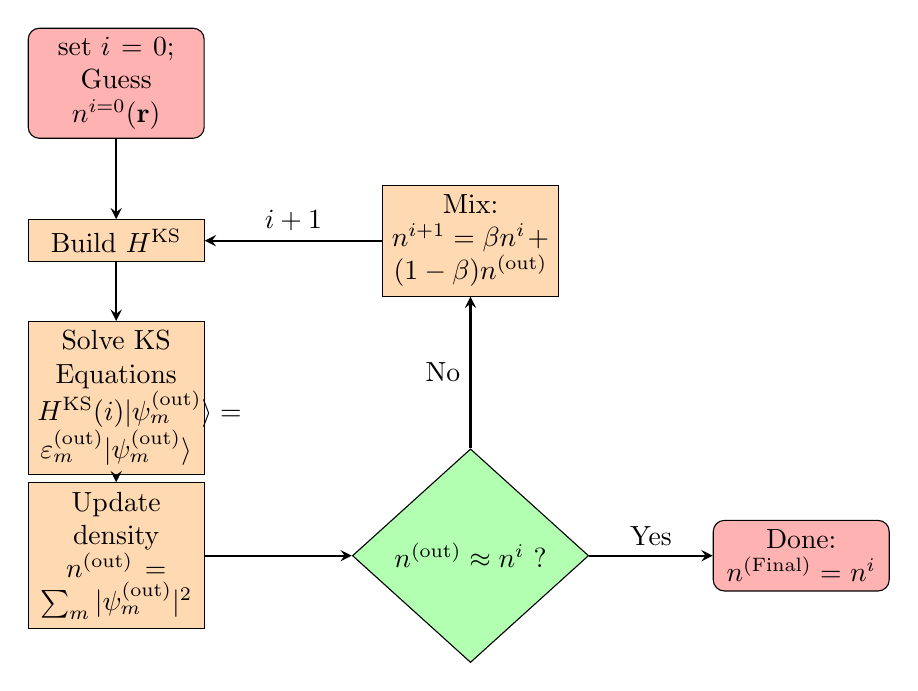
\begin{tikzpicture}[node distance=2cm]
\node (start) [startstop] 
   {set $i=0$; Guess $n^{i=0}(\mathbf{r})$};
\node (HKS) [process, below of=start] 
   {Build $H^\mathrm{KS}$};
\node (solve) [process, below of=HKS] 
   {Solve KS Equations $H^\mathrm{KS}(i)\vert \psi_m^\mathrm{(out)} \rangle 
   = \varepsilon_m^\mathrm{(out)}\vert\psi_m^\mathrm{(out)} \rangle$};
\node (update) [process, below of=solve] 
   {Update density $n^\mathrm{(out)} = \sum_m\vert \psi_m^\mathrm{(out)} \vert ^2$};
\node (check) [decision, right of=update, xshift=2.5cm] 
   {$n^\mathrm{(out)} \approx n^i$ ?};
\node (mix) [process, right of=HKS, xshift=2.5cm] 
   {Mix: $n^{i+1} = \beta n^i + (1-\beta)n^\mathrm{(out)}$};
\node (done) [startstop, right of=check, xshift=2.2cm]
   {Done: $n^\mathrm{(Final)} = n^i$};

\draw [arrow] (start) -- (HKS);
\draw [arrow] (HKS) -- (solve);
\draw [arrow] (solve) -- (update);
\draw [arrow] (update) -- (check);
\draw [arrow] (check) -- node[anchor=east]{No} (mix);
\draw [arrow]  (mix) -- node[anchor=south]{$i+1$} (HKS);
\draw [arrow] (check) -- node[anchor=south]{Yes} (done);
 
\end{tikzpicture}

\end{frame}

\begin{frame}
\footnotesize
\frametitle{The self-consistency cycle}

\onslide<1->{
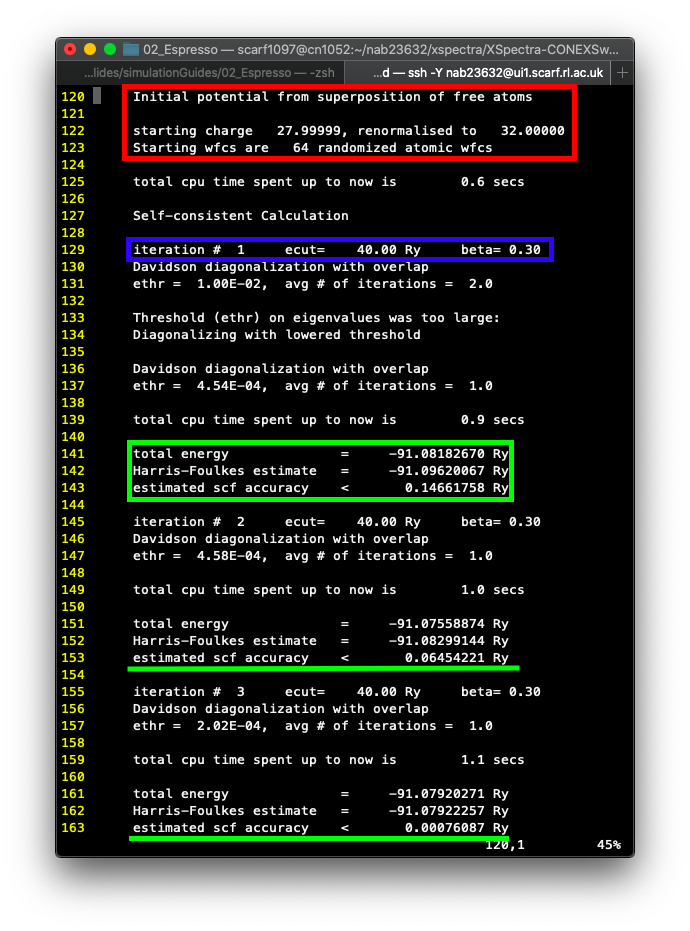
\includegraphics[height=0.8\textheight]{Figure/start_scf.png}
}
\onslide<2->{
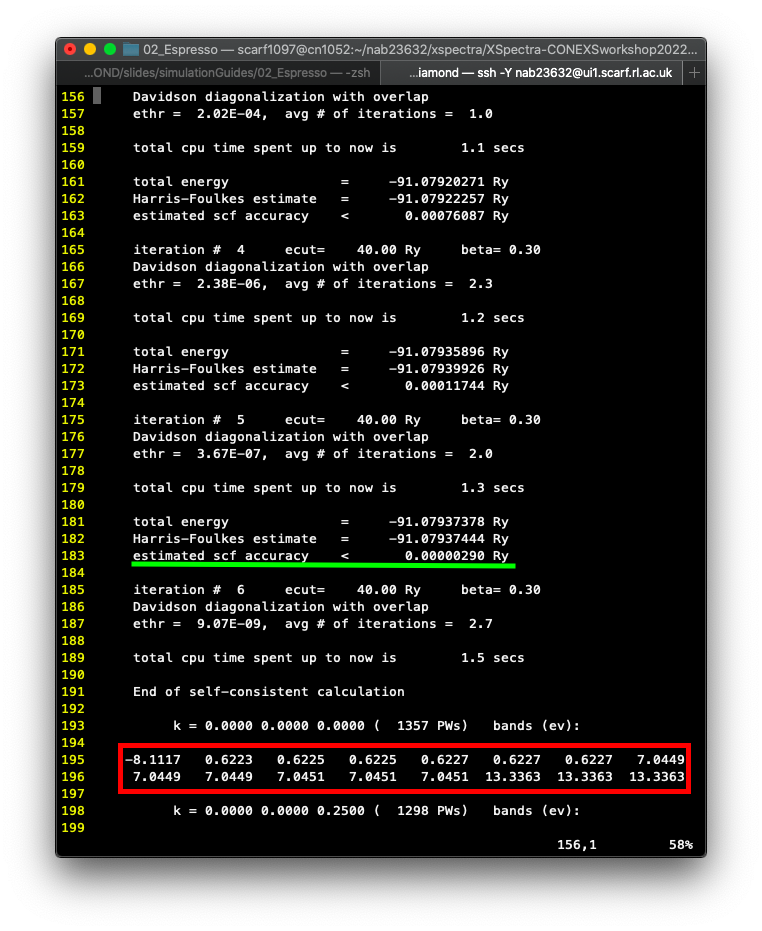
\includegraphics[height=0.8\textheight]{Figure/end_scf.png}
}

\end{frame}

\section{The Basis Set}

\begin{frame}
\footnotesize
\frametitle{Introduction to basis sets (General)}

\begin{equation}
\psi_i(\mathbf{r}) = \sum_\alpha^M c_\alpha \phi_\alpha(\mathbf{r})
\end{equation}

\begin{center}
\begin{minipage}{0.95\textwidth}
\begin{itemize}
\item[{$\psi_i(\mathbf{r})$}:] The function that we want to represent (KS wfn)
\item[{$\phi_\alpha(\mathbf{r})$}:] The set of basis functions
\begin{itemize}
\item[$\rightarrow$] Predefined (known) functions
\item[$\rightarrow$] Determine choice of code
\end{itemize}
\item[{$M$}:] The size of the basis set
\item[{$C_\alpha$}:] Expansion Coefficients
\begin{itemize}
\item[$\rightarrow$] Information stored on the computer
\item[$\rightarrow$] Want to keep M as small as possible
\item[$\rightarrow$] More $C_\alpha$ means more complete basis set (more transferable)
\end{itemize}
\end{itemize}
\end{minipage}
\end{center}

\end{frame}

\end{document}
